\documentclass{beamer}
\usepackage{graphicx}
\usepackage{movie15}
\usepackage{caption}
\newcommand\FourQuad[4]{%
    \begin{minipage}[b][.35\textheight][t]{.47\textwidth}#1\end{minipage}\hfill%
    \begin{minipage}[b][.35\textheight][t]{.47\textwidth}#2\end{minipage}\\[0.5em]
    \begin{minipage}[b][.35\textheight][t]{.47\textwidth}#3\end{minipage}\hfill
    \begin{minipage}[b][.35\textheight][t]{.47\textwidth}#4\end{minipage}%
    }
\usepackage{subcaption}
\usepackage{xcolor}
\usepackage{float}
\usepackage[T1]{fontenc}
\usepackage{mathtools}
\usepackage[english]{babel}
\usepackage{animate}
\usepackage{comment}
\usetheme{Ilmenau}
\beamertemplatenavigationsymbolsempty

\title{Delayed Monetary Incentive Reward Task}

\date{\today}

\title[{\makebox[.953\paperwidth]{Delayed Monetary Incentive Reward Task\hfill%
\insertframenumber/\inserttotalframenumber}}]{Delayed Monetary Incentive Reward Task}

\begin{document}

\begin{frame}
\titlepage
\end{frame}

\begin{frame}
\frametitle{General Overview}
	\begin{itemize}
		\item 2 conditions (blocks)
			\begin{itemize}
				\item Reward
					\begin{itemize}
						\item 135 reward trials; 45 neutral trials
					\end{itemize}
				\item Neutral
					\begin{itemize}
						\item 45 reward trials; 135 neutral trials
					\end{itemize}
			\end{itemize}
		\item Each lasted 36 minutes in Schott paper
		\item But they did PET over 2 days!
		\item So, I suppose we would aim for approximately 20 minute blocks?
	\end{itemize}
\end{frame}

\begin{section}{review of task}
\begin{frame}
\frametitle{Reward Condition}
\begin{center}
\bf{Reward Trial} \\
	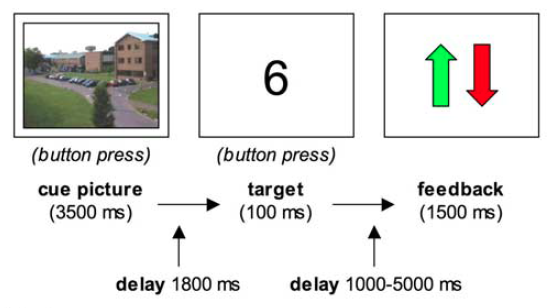
\includegraphics[height=38mm,width=62mm]{rewardcond} \\
	\begin{itemize}
		\footnotesize{
		\item In this example, outdoor scene is reward cue (counterbalanced with indoor scene across subjects)
		\item See green arrow if correct (~80\%) of trials 
		\item See red arrow if incorrect or too slow to respond; (~20\%) of trials 
		\item Gain 50 cents on correct trials; lose 20 cents on incorrect trials}
	\end{itemize}
\end{center}
\end{frame}

\begin{frame}
\frametitle{Reward Condition}
\begin{center}
\bf{Neutral Trial} \\
	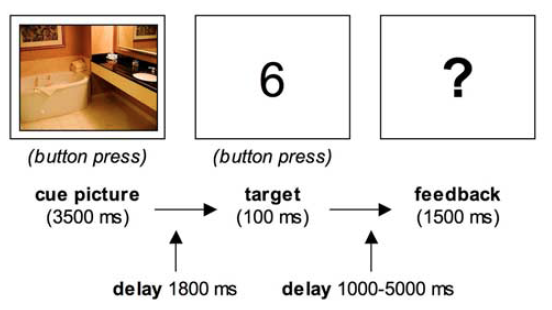
\includegraphics[height=38mm,width=62mm]{neutralcond} \\
	\begin{itemize}
		\footnotesize{
		\item  In this example, indoor scene is neutral cue (counterbalanced with outdoor scene across subjects)
		\item Always see a question mark as the outcome }
	\end{itemize}
\end{center}
\end{frame}

\begin{frame}
\frametitle{Neutral Condition}
\begin{center}
\bf{Reward Trial - Bogus!} \\
	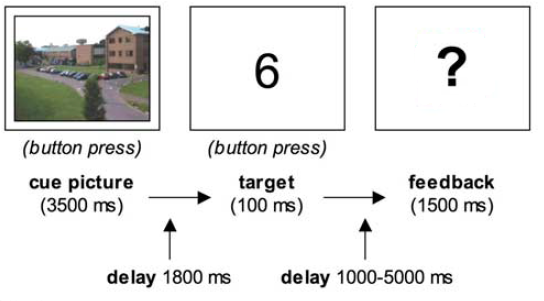
\includegraphics[height=38mm,width=62mm]{bogusrewardcond} \\
	\begin{itemize}
		\footnotesize{
		\item In this example, outdoor scene is reward cue (counterbalanced with indoor scene across subjects)
		\item But subjects see a question mark as the outcome! - Bogus! }
	\end{itemize}
\end{center}
\end{frame}

\begin{frame}
\frametitle{Neutral Condition}
\begin{center}
\bf{Neutral Trial} \\
	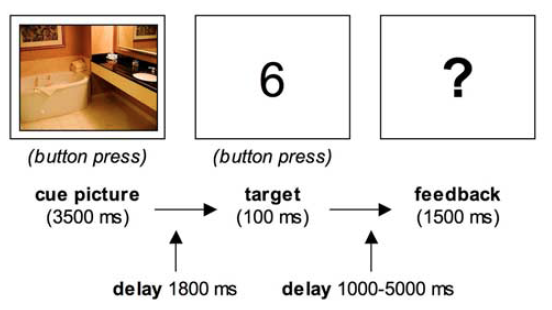
\includegraphics[height=38mm,width=62mm]{neutralcond} \\
	\begin{itemize}
		\footnotesize{
		\item In this example, indoor scene is neutral cue (counterbalanced with outdoor scene across subjects)
		\item Always see a question mark as the outcome }
	\end{itemize}
\end{center}
\end{frame}

\begin{frame}
\frametitle{Some Important Notes}
\begin{itemize}
    {\small 
	\item Subjects responded with a button press to indicate whether the saw an indoor or outdoor scene during cue phase
	\item Neutral condition contains inverse trial structure from reward condition to minimize sensorimotor and cognitive processing differences
	\item Subjects were explicitly told the trial structure of the blocks.
	}
\end{itemize}
\end{frame}

\begin{frame}
\frametitle{Lingering Quesitons}
	\begin{itemize}
		\item Block Length?
		\item Jitter in between cue and number comparison?
	\end{itemize}
\end{frame}
\end{section}
%%%%%%%%%%%%%%%%%%%%%%%%%%%%%%%%%%%
% NOW for a simulation of the task%
%%%%%%%%%%%%%%%%%%%%%%%%%%%%%%%%%%%
\begin{section}{task presentation: reward block}
\begin{subsection}{reward block - reward correct}
%%%% INDOOR=reward correct
\begin{frame} \frametitle{REWARD (correct)} here indoor is the reward cue \end{frame}
\begin{frame} \frametitle{CUE for 3.5s}
   \begin{center}
	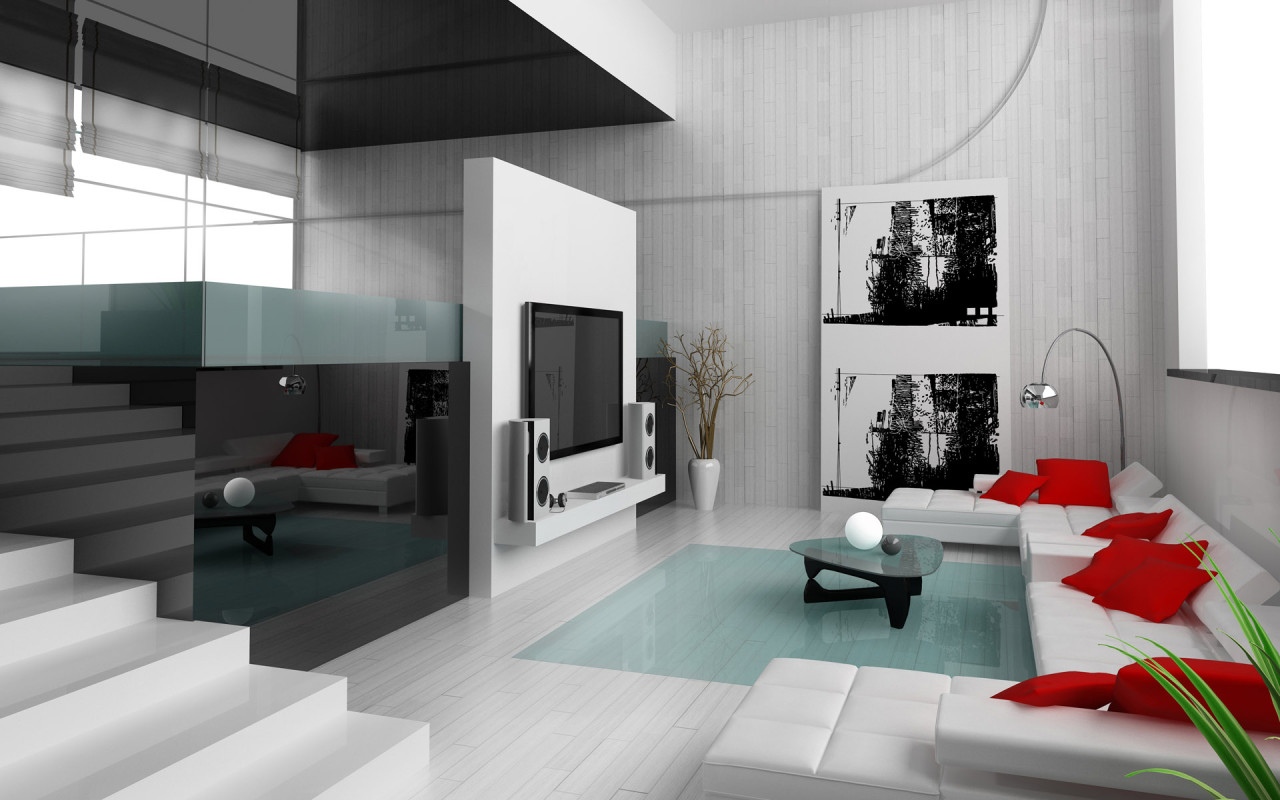
\includegraphics[width=.5\textwidth]{../imgs/Scenes/Indoors/living-room-interior-design.jpg} \\
   \end{center}
\end{frame}

\begin{frame} \frametitle{1.8s wait} \end{frame}
\begin{frame} \frametitle{Number for 0.1s} \center{\huge{2}} \end{frame}
\begin{frame} \frametitle{variable response window (80\% correct)} \tiny{you respond correctly and in time} \end{frame}
\begin{frame} \frametitle{wait for 1 to 6 secs} \end{frame}
\begin{frame} 
 \frametitle{see reward/loss for 1.5s}
   \begin{center}
	  %
\includegraphics[width=.5\textwidth]{../imgs/Scenes/Indoors/he.jpg} \\
     \center{\textcolor{green}{\huge{$\uparrow$}}}
   \end{center}
\end{frame}
\end{subsection}
%%%% END reward correct


%%%% INDOOR=reward incorrect
\begin{subsection}{reward block - reward incorrect}
\begin{frame} \frametitle{REWARD (incorrect)} here indoor is the reward cue \end{frame}
\begin{frame} \frametitle{CUE for 3.5s}
   \begin{center}
	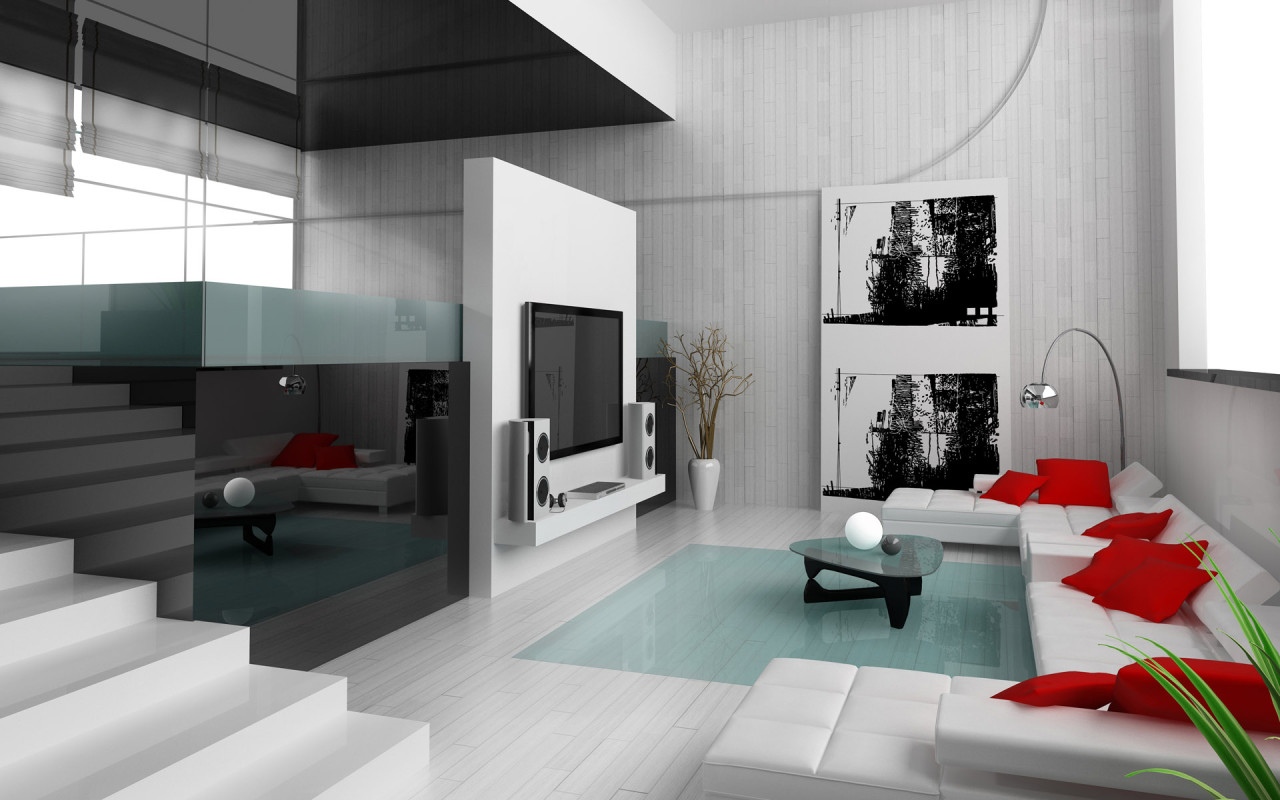
\includegraphics[width=.5\textwidth]{../imgs/Scenes/Indoors/living-room-interior-design.jpg} \\
   \end{center}
\end{frame}

\begin{frame} \frametitle{1.8s wait} \end{frame}
\begin{frame} \frametitle{Number for 0.1s} \center{\huge{4}} \end{frame}
\begin{frame} \frametitle{variable response window (80\% correct)} \tiny{you respond incorrectly or not in time} \end{frame}
\begin{frame} \frametitle{wait for 1 to 6 secs} \end{frame}
\begin{frame} 
 \frametitle{see reward/loss for 1.5s}
   \begin{center}
     \center{\textcolor{red}{\huge{$\downarrow$}}}
   \end{center}
\end{frame}
\end{subsection}
%%%% END reward loss



%%%% OUTDOOR=neutral incorrect
\begin{subsection}{reward block - neutral}
\begin{frame} \frametitle{NEUTRAL} here outdoor is the neutral/unrewarded cue \end{frame}
\begin{frame} \frametitle{CUE for 3.5s}
   \begin{center}
	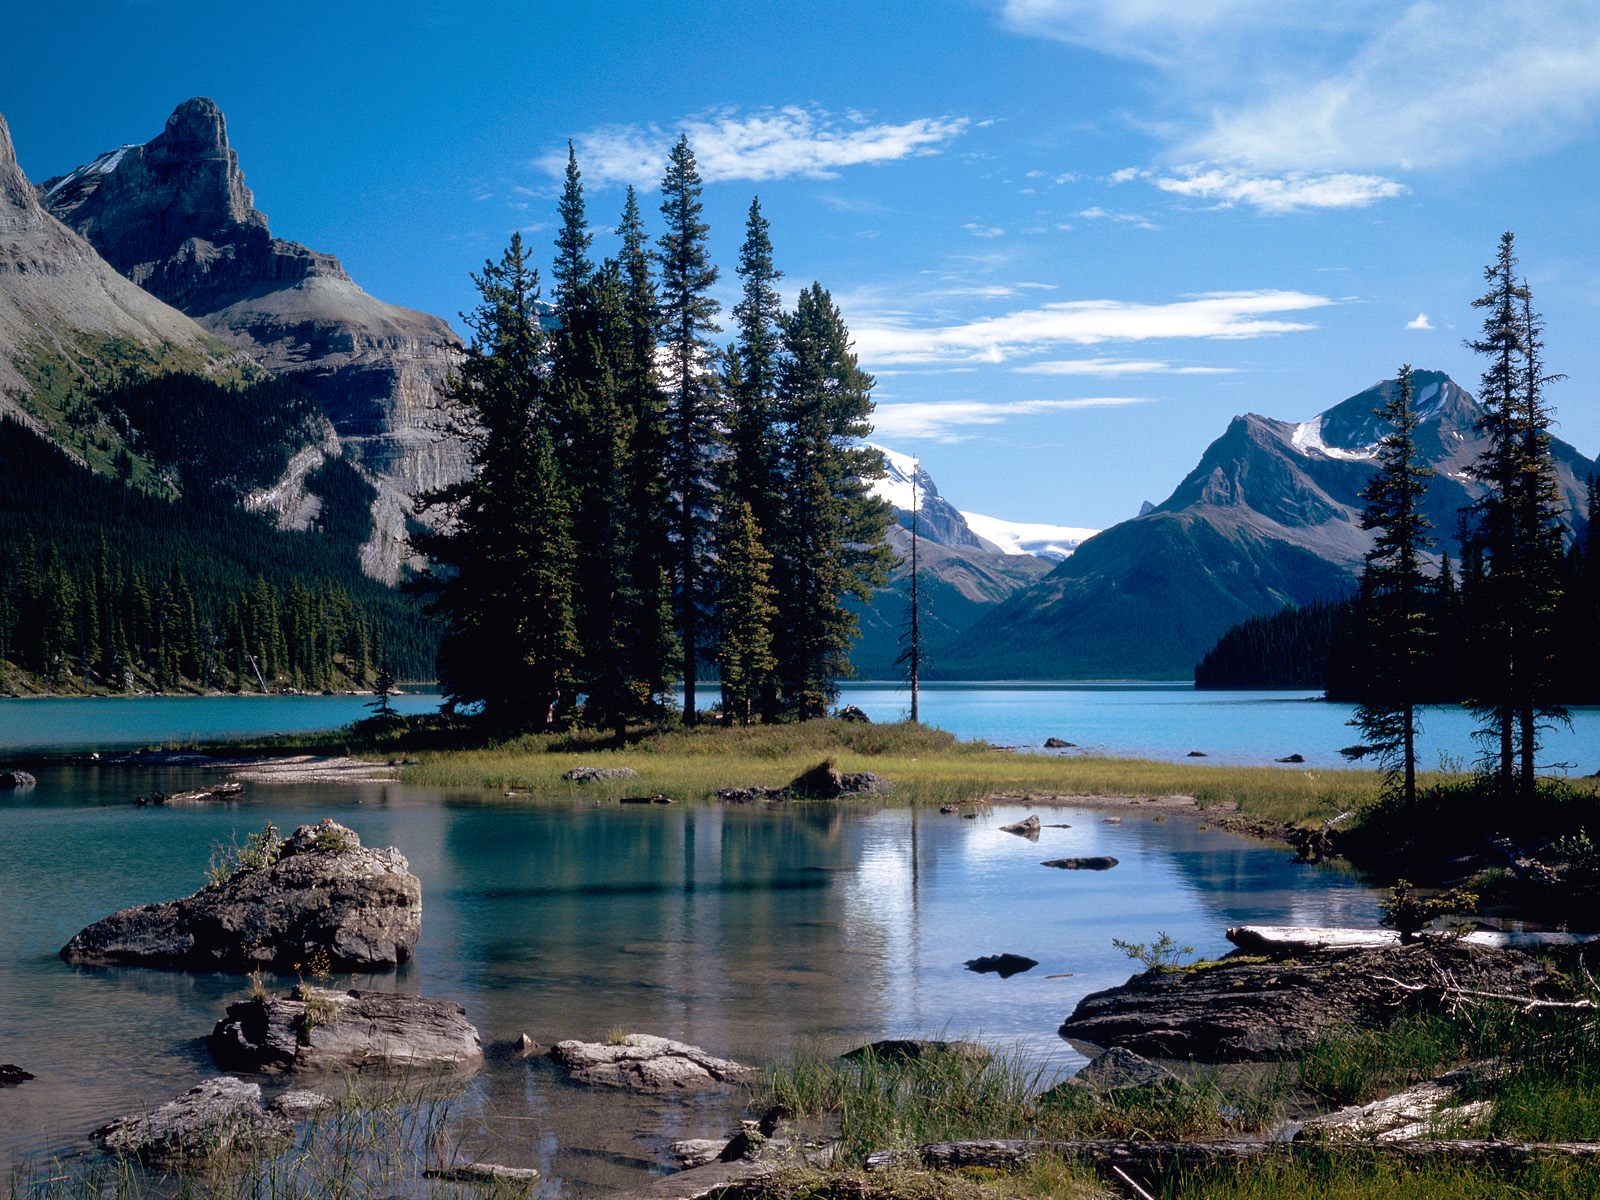
\includegraphics[width=.5\textwidth]{../imgs/Scenes/Outdoors/the-great-outdoors.jpg} \\
   \end{center}
\end{frame}

\begin{frame} \frametitle{1.8s wait} \end{frame}
\begin{frame} \frametitle{Number for 0.1s} \center{\huge{6}} \end{frame}
\begin{frame} \frametitle{wait for 1 to 6 secs} \tiny{response doesn't matter}\end{frame}
\begin{frame} 
 \frametitle{see reward/loss for 1.5s}
   \begin{center}
     \center{\huge{?}}
   \end{center}
\end{frame}
%%%% END neutral loss

\end{subsection}
\end{section}





%%%%%%%%%%%%%%%%%%% NEUTRAL BLOCK
\begin{section}{task presentation: neutral block}
\begin{subsection}{neutral block - reward correct}
%%%% INDOOR=reward correct
\begin{frame} \frametitle{REWARD (correct)} here indoor is the reward cue \end{frame}
\begin{frame} \frametitle{CUE for 3.5s}
   \begin{center}
	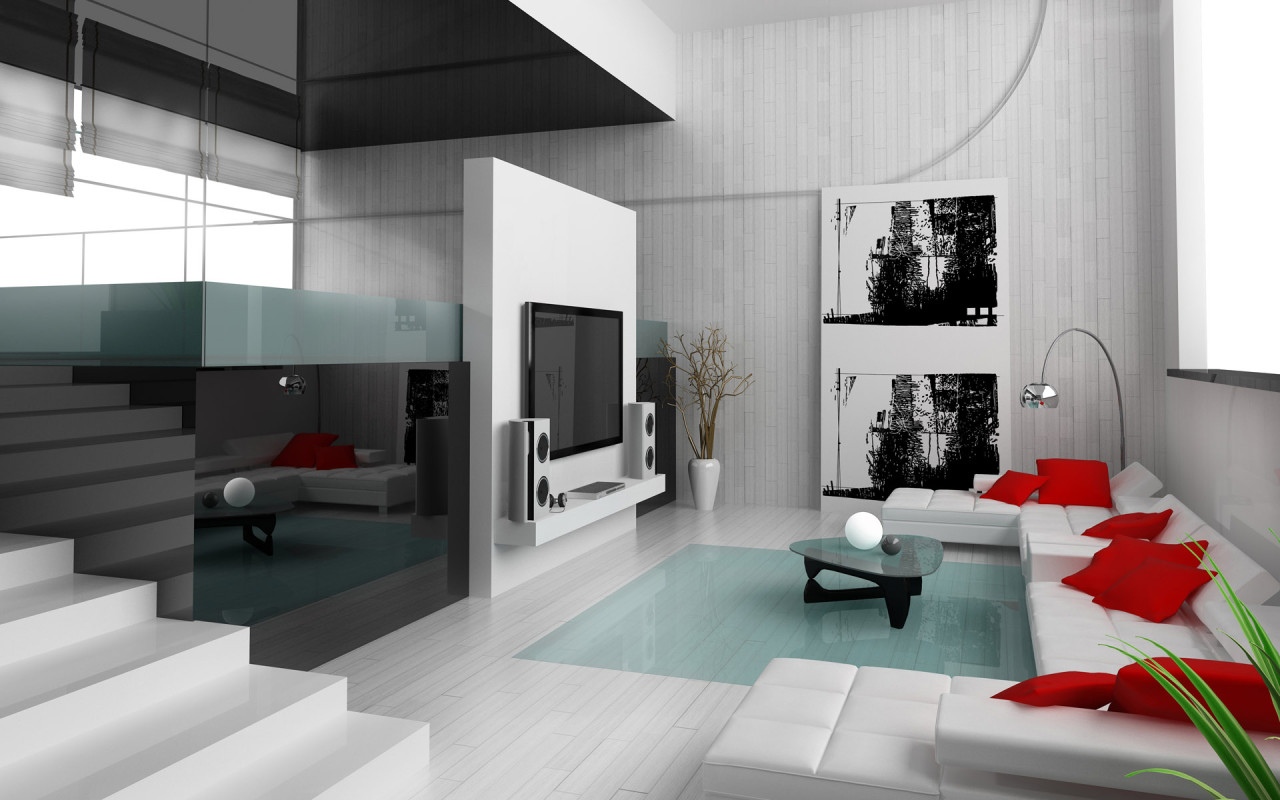
\includegraphics[width=.5\textwidth]{../imgs/Scenes/Indoors/living-room-interior-design.jpg} \\
   \end{center}
\end{frame}

\begin{frame} \frametitle{1.8s wait} \end{frame}
\begin{frame} \frametitle{Number for 0.1s} \center{\huge{2}} \end{frame}
\begin{frame} \frametitle{wait for 1 to 6 secs} \end{frame}
\begin{frame} 
 \frametitle{see reward/loss for 1.5s}
   \begin{center}
	  %
\includegraphics[width=.5\textwidth]{../imgs/Scenes/Indoors/he.jpg} \\
     \center{\huge{?}}
   \end{center}
\end{frame}
\end{subsection}
%%%% END reward correct



%%%% OUTDOOR=neutral incorrect
\begin{subsection}{neutral block - neutral}
\begin{frame} \frametitle{NEUTRAL} here outdoor is the neutral/unrewarded cue \end{frame}
\begin{frame} \frametitle{CUE for 3.5s}
   \begin{center}
	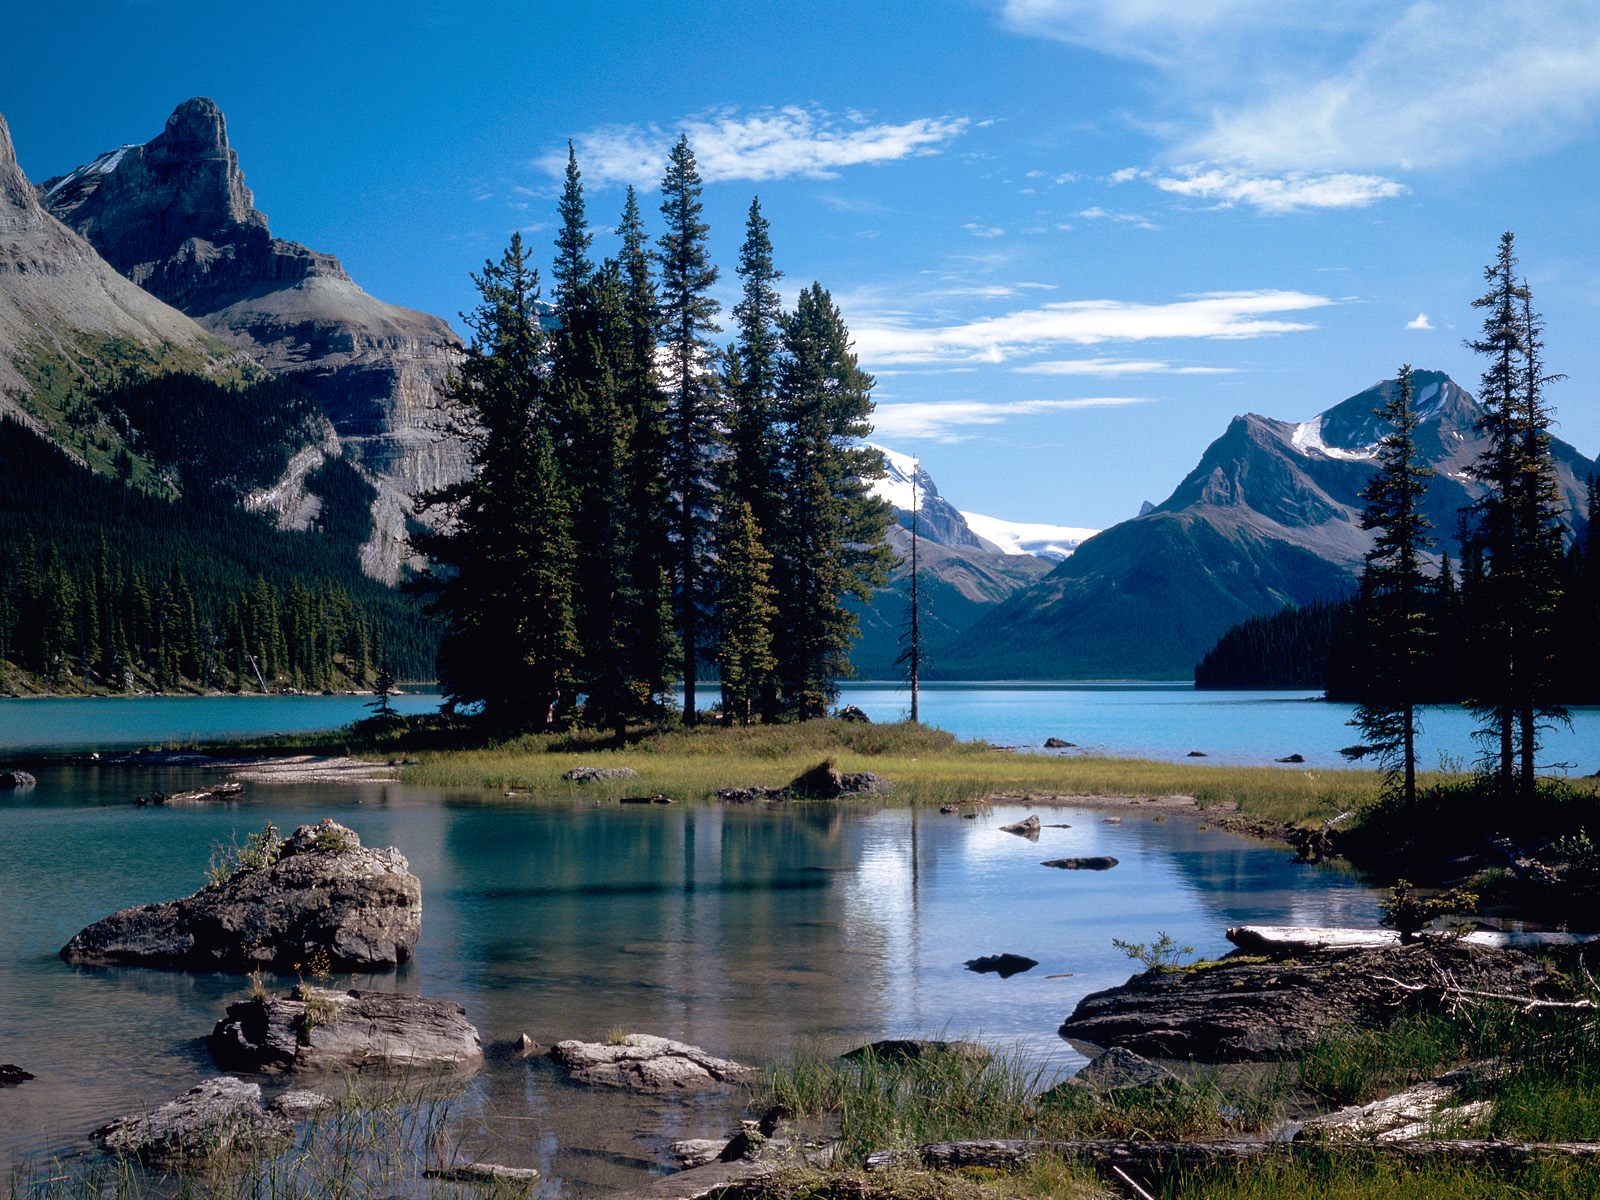
\includegraphics[width=.5\textwidth]{../imgs/Scenes/Outdoors/the-great-outdoors.jpg} \\
   \end{center}
\end{frame}

\begin{frame} \frametitle{1.8s wait} \end{frame}
\begin{frame} \frametitle{Number for 0.1s} \center{\huge{8}} \end{frame}
\begin{frame} \frametitle{wait for 1 to 6 secs} \tiny{response doesn't matter}\end{frame}
\begin{frame} 
 \frametitle{see reward/loss for 1.5s}
   \begin{center}
     \center{\huge{?}}
   \end{center}
\end{frame}
%%%% END neutral loss

\end{subsection}
\end{section}

\end{document}
